\documentclass[]{article}
\usepackage{lmodern}
\usepackage{amssymb,amsmath}
\usepackage{ifxetex,ifluatex}
\usepackage{fixltx2e} % provides \textsubscript
\ifnum 0\ifxetex 1\fi\ifluatex 1\fi=0 % if pdftex
  \usepackage[T1]{fontenc}
  \usepackage[utf8]{inputenc}
\else % if luatex or xelatex
  \ifxetex
    \usepackage{mathspec}
  \else
    \usepackage{fontspec}
  \fi
  \defaultfontfeatures{Ligatures=TeX,Scale=MatchLowercase}
\fi
% use upquote if available, for straight quotes in verbatim environments
\IfFileExists{upquote.sty}{\usepackage{upquote}}{}
% use microtype if available
\IfFileExists{microtype.sty}{%
\usepackage{microtype}
\UseMicrotypeSet[protrusion]{basicmath} % disable protrusion for tt fonts
}{}
\usepackage[margin=1in]{geometry}
\usepackage{hyperref}
\hypersetup{unicode=true,
            pdftitle={CKiD research project},
            pdfauthor={Benjamin Matta, MD},
            pdfborder={0 0 0},
            breaklinks=true}
\urlstyle{same}  % don't use monospace font for urls
\usepackage{color}
\usepackage{fancyvrb}
\newcommand{\VerbBar}{|}
\newcommand{\VERB}{\Verb[commandchars=\\\{\}]}
\DefineVerbatimEnvironment{Highlighting}{Verbatim}{commandchars=\\\{\}}
% Add ',fontsize=\small' for more characters per line
\usepackage{framed}
\definecolor{shadecolor}{RGB}{248,248,248}
\newenvironment{Shaded}{\begin{snugshade}}{\end{snugshade}}
\newcommand{\AlertTok}[1]{\textcolor[rgb]{0.94,0.16,0.16}{#1}}
\newcommand{\AnnotationTok}[1]{\textcolor[rgb]{0.56,0.35,0.01}{\textbf{\textit{#1}}}}
\newcommand{\AttributeTok}[1]{\textcolor[rgb]{0.77,0.63,0.00}{#1}}
\newcommand{\BaseNTok}[1]{\textcolor[rgb]{0.00,0.00,0.81}{#1}}
\newcommand{\BuiltInTok}[1]{#1}
\newcommand{\CharTok}[1]{\textcolor[rgb]{0.31,0.60,0.02}{#1}}
\newcommand{\CommentTok}[1]{\textcolor[rgb]{0.56,0.35,0.01}{\textit{#1}}}
\newcommand{\CommentVarTok}[1]{\textcolor[rgb]{0.56,0.35,0.01}{\textbf{\textit{#1}}}}
\newcommand{\ConstantTok}[1]{\textcolor[rgb]{0.00,0.00,0.00}{#1}}
\newcommand{\ControlFlowTok}[1]{\textcolor[rgb]{0.13,0.29,0.53}{\textbf{#1}}}
\newcommand{\DataTypeTok}[1]{\textcolor[rgb]{0.13,0.29,0.53}{#1}}
\newcommand{\DecValTok}[1]{\textcolor[rgb]{0.00,0.00,0.81}{#1}}
\newcommand{\DocumentationTok}[1]{\textcolor[rgb]{0.56,0.35,0.01}{\textbf{\textit{#1}}}}
\newcommand{\ErrorTok}[1]{\textcolor[rgb]{0.64,0.00,0.00}{\textbf{#1}}}
\newcommand{\ExtensionTok}[1]{#1}
\newcommand{\FloatTok}[1]{\textcolor[rgb]{0.00,0.00,0.81}{#1}}
\newcommand{\FunctionTok}[1]{\textcolor[rgb]{0.00,0.00,0.00}{#1}}
\newcommand{\ImportTok}[1]{#1}
\newcommand{\InformationTok}[1]{\textcolor[rgb]{0.56,0.35,0.01}{\textbf{\textit{#1}}}}
\newcommand{\KeywordTok}[1]{\textcolor[rgb]{0.13,0.29,0.53}{\textbf{#1}}}
\newcommand{\NormalTok}[1]{#1}
\newcommand{\OperatorTok}[1]{\textcolor[rgb]{0.81,0.36,0.00}{\textbf{#1}}}
\newcommand{\OtherTok}[1]{\textcolor[rgb]{0.56,0.35,0.01}{#1}}
\newcommand{\PreprocessorTok}[1]{\textcolor[rgb]{0.56,0.35,0.01}{\textit{#1}}}
\newcommand{\RegionMarkerTok}[1]{#1}
\newcommand{\SpecialCharTok}[1]{\textcolor[rgb]{0.00,0.00,0.00}{#1}}
\newcommand{\SpecialStringTok}[1]{\textcolor[rgb]{0.31,0.60,0.02}{#1}}
\newcommand{\StringTok}[1]{\textcolor[rgb]{0.31,0.60,0.02}{#1}}
\newcommand{\VariableTok}[1]{\textcolor[rgb]{0.00,0.00,0.00}{#1}}
\newcommand{\VerbatimStringTok}[1]{\textcolor[rgb]{0.31,0.60,0.02}{#1}}
\newcommand{\WarningTok}[1]{\textcolor[rgb]{0.56,0.35,0.01}{\textbf{\textit{#1}}}}
\usepackage{longtable,booktabs}
\usepackage{graphicx,grffile}
\makeatletter
\def\maxwidth{\ifdim\Gin@nat@width>\linewidth\linewidth\else\Gin@nat@width\fi}
\def\maxheight{\ifdim\Gin@nat@height>\textheight\textheight\else\Gin@nat@height\fi}
\makeatother
% Scale images if necessary, so that they will not overflow the page
% margins by default, and it is still possible to overwrite the defaults
% using explicit options in \includegraphics[width, height, ...]{}
\setkeys{Gin}{width=\maxwidth,height=\maxheight,keepaspectratio}
\IfFileExists{parskip.sty}{%
\usepackage{parskip}
}{% else
\setlength{\parindent}{0pt}
\setlength{\parskip}{6pt plus 2pt minus 1pt}
}
\setlength{\emergencystretch}{3em}  % prevent overfull lines
\providecommand{\tightlist}{%
  \setlength{\itemsep}{0pt}\setlength{\parskip}{0pt}}
\setcounter{secnumdepth}{0}
% Redefines (sub)paragraphs to behave more like sections
\ifx\paragraph\undefined\else
\let\oldparagraph\paragraph
\renewcommand{\paragraph}[1]{\oldparagraph{#1}\mbox{}}
\fi
\ifx\subparagraph\undefined\else
\let\oldsubparagraph\subparagraph
\renewcommand{\subparagraph}[1]{\oldsubparagraph{#1}\mbox{}}
\fi

%%% Use protect on footnotes to avoid problems with footnotes in titles
\let\rmarkdownfootnote\footnote%
\def\footnote{\protect\rmarkdownfootnote}

%%% Change title format to be more compact
\usepackage{titling}

% Create subtitle command for use in maketitle
\newcommand{\subtitle}[1]{
  \posttitle{
    \begin{center}\large#1\end{center}
    }
}

\setlength{\droptitle}{-2em}

  \title{CKiD research project}
    \pretitle{\vspace{\droptitle}\centering\huge}
  \posttitle{\par}
    \author{Benjamin Matta, MD}
    \preauthor{\centering\large\emph}
  \postauthor{\par}
      \predate{\centering\large\emph}
  \postdate{\par}
    \date{December 22, 2018}


\begin{document}
\maketitle

\hypertarget{do-higher-cumulative-antihypertensive-doses-result-in-better-blood-pressure-bp-control-in-children-with-chronic-kidney-disease-ckd}{%
\section{Do higher cumulative antihypertensive doses result in better
blood pressure (BP) control in children with chronic kidney disease
(CKD)?}\label{do-higher-cumulative-antihypertensive-doses-result-in-better-blood-pressure-bp-control-in-children-with-chronic-kidney-disease-ckd}}

\hypertarget{study-population-n255}{%
\subsection{Study population (n=255)}\label{study-population-n255}}

\hypertarget{inclusion-criteria}{%
\subsubsection{Inclusion criteria}\label{inclusion-criteria}}

\begin{itemize}
\tightlist
\item
  entered into CKiD study
\item
  visit 20
\item
  measured BP
\item
  known age, gender and height
\item
  successful BPM study
\item
  eGFR based on full CkiD gfr equation
  \[ eGFR = 39.8 \times \left ( \frac{ht(m)}{Scr} \right )^{0.456} \times \left( \frac{1.8}{cysC} \right )^{0.418}\times \left ( \frac{30}{BUN} \right )^{0.079}\times 1.076^{male}\times \left ( \frac{ht(m)}{1.4} \right )^{0.179} \]
\end{itemize}

\hypertarget{exclusion-criteria}{%
\subsubsection{Exclusion criteria}\label{exclusion-criteria}}

\begin{itemize}
\tightlist
\item
  missing BP medication details:

  \begin{itemize}
  \tightlist
  \item
    daily dose
  \item
    daily frequency
  \item
    weight
  \end{itemize}
\end{itemize}

\hypertarget{definition-of-drug-dose-index-ddi}{%
\subsubsection{Definition of Drug Dose Index
(DDI)}\label{definition-of-drug-dose-index-ddi}}

\begin{itemize}
\tightlist
\item
  The DDI is a property of every drug dose and depends on

  \begin{itemize}
  \tightlist
  \item
    the medication
  \item
    the maximum dose based on the patient's age, weight and eGFR
  \end{itemize}
\item
  The DDI is the ratio of the patient's dose to the maximum dose
  appropriate for that patient, up to a value of 1
  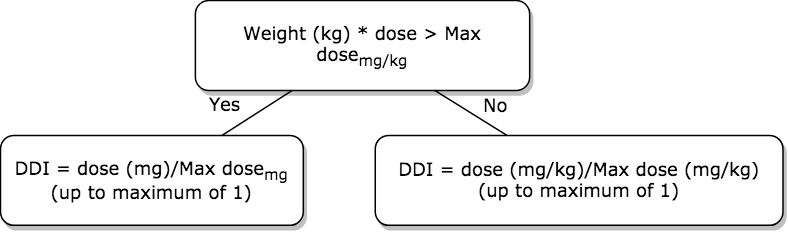
\includegraphics{results/DDI_algorithm.png}
\end{itemize}

\hypertarget{load-the-data}{%
\subsection{Load the data}\label{load-the-data}}

File=``test3.RData''

\hypertarget{define-study-population-and-show-summary}{%
\section{Define study population and show
summary}\label{define-study-population-and-show-summary}}

\begin{Shaded}
\begin{Highlighting}[]
\CommentTok{# define study population}
\NormalTok{combo_cases<-medsum_full.old }\OperatorTok\StringTok{ }\KeywordTok{filter}\NormalTok{(VISIT}\OperatorTok{==}\DecValTok{20}\NormalTok{,}\KeywordTok{length}\NormalTok{(}\KeywordTok{grep}\NormalTok{(}\StringTok{"}\CharTok{\textbackslash{}\textbackslash{}}\StringTok{/"}\NormalTok{,med.corrected)}\OperatorTok{!=}\NormalTok{0L)) }\OperatorTok\StringTok{ }\KeywordTok{ungroup}\NormalTok{() }\OperatorTok\StringTok{ }\KeywordTok{select}\NormalTok{(CASEID) }\OperatorTok\StringTok{ }\KeywordTok{unique}\NormalTok{() }\OperatorTok\StringTok{ }\KeywordTok{unlist}\NormalTok{() }\OperatorTok\StringTok{ }\KeywordTok{as.numeric}\NormalTok{()}
\NormalTok{cases<-test }\OperatorTok\StringTok{ }\KeywordTok{filter}\NormalTok{(}\OperatorTok{!}\NormalTok{CASEID }\OperatorTok\StringTok{ }\NormalTok{combo_cases,VISIT}\OperatorTok{==}\DecValTok{20}\NormalTok{, n_agents}\OperatorTok{>}\DecValTok{0}\NormalTok{,}\OperatorTok{!}\KeywordTok{is.na}\NormalTok{(sum_DDI),ABPMSUCCESS}\OperatorTok{==}\DecValTok{1}\NormalTok{,}\OperatorTok{!}\NormalTok{BPclass.factor}\OperatorTok{==}\StringTok{"WCH"}\NormalTok{,}\OperatorTok{!}\KeywordTok{is.na}\NormalTok{(BUN), }\OperatorTok{!}\KeywordTok{is.na}\NormalTok{(CYC_DB),}\OperatorTok{!}\KeywordTok{is.na}\NormalTok{(SCR),}\OperatorTok{!}\KeywordTok{is.na}\NormalTok{(AVHEIGHT), }\OperatorTok{!}\KeywordTok{is.na}\NormalTok{(AVWEIGHT), }\OperatorTok{!}\KeywordTok{is.na}\NormalTok{(BPstatus2017)) }\OperatorTok\StringTok{ }\KeywordTok{ungroup}\NormalTok{() }\OperatorTok\KeywordTok{select}\NormalTok{(CASEID) }\OperatorTok\StringTok{ }\NormalTok{unique }\OperatorTok\StringTok{ }\NormalTok{unlist }\OperatorTok\StringTok{ }\KeywordTok{as.numeric}\NormalTok{()}\CommentTok{# exclude those taking combo medications}
\NormalTok{test.cohort<-test }\OperatorTok\StringTok{ }\KeywordTok{filter}\NormalTok{(VISIT}\OperatorTok{==}\DecValTok{20}\NormalTok{, CASEID }\OperatorTok\StringTok{ }\NormalTok{cases)}

\NormalTok{test.cohort<-test.cohort }\OperatorTok\StringTok{ }\KeywordTok{mutate}\NormalTok{(}\DataTypeTok{sum_DDI.ln=}\KeywordTok{log}\NormalTok{(sum_DDI))}
\KeywordTok{library}\NormalTok{(summarytools)}
\KeywordTok{dfSummary}\NormalTok{(}\DataTypeTok{plain.ascii=} \OtherTok{FALSE}\NormalTok{,}\DataTypeTok{style =} \StringTok{"grid"}\NormalTok{,test.cohort }\OperatorTok\StringTok{ }\KeywordTok{select}\NormalTok{(age,MALE1FE0,CKD_stage,gfr,CKDONST,n_agents,BPclass.factor,SBPZAGH2017,DBPPCTAGH2017, LVMIp,Upc,Upc.factor,BMIz,GNGDIAG,GHTOTINC,RACE,sum_DDI))}
\end{Highlighting}
\end{Shaded}

\hypertarget{data-frame-summary}{%
\subsubsection{Data Frame Summary}\label{data-frame-summary}}

\textbf{test.cohort}\\
\textbf{Dimensions:} 255 x 17\\
\textbf{Duplicates:} 0

\begin{longtable}[]{@{}lllllll@{}}
\toprule
\begin{minipage}[b]{0.03\columnwidth}\raggedright
No\strut
\end{minipage} & \begin{minipage}[b]{0.13\columnwidth}\raggedright
Variable\strut
\end{minipage} & \begin{minipage}[b]{0.22\columnwidth}\raggedright
Stats / Values\strut
\end{minipage} & \begin{minipage}[b]{0.14\columnwidth}\raggedright
Freqs (\% of Valid)\strut
\end{minipage} & \begin{minipage}[b]{0.14\columnwidth}\raggedright
Text Graph\strut
\end{minipage} & \begin{minipage}[b]{0.07\columnwidth}\raggedright
Valid\strut
\end{minipage} & \begin{minipage}[b]{0.07\columnwidth}\raggedright
Missing\strut
\end{minipage}\tabularnewline
\midrule
\endhead
\begin{minipage}[t]{0.03\columnwidth}\raggedright
1\strut
\end{minipage} & \begin{minipage}[t]{0.13\columnwidth}\raggedright
age\\
{[}numeric{]}\strut
\end{minipage} & \begin{minipage}[t]{0.22\columnwidth}\raggedright
Mean (Std.Dev) :12.85 (3.68)\\
min \textless{} med \textless{} max:\\
3.01 \textless{} 13.04 \textless{} 19.45\\
IQR (CV) :5.98 (0.29)\strut
\end{minipage} & \begin{minipage}[t]{0.14\columnwidth}\raggedright
229 distinct values\strut
\end{minipage} & \begin{minipage}[t]{0.14\columnwidth}\raggedright
\strut
\end{minipage} & \begin{minipage}[t]{0.07\columnwidth}\raggedright
255\\
(100\%)\strut
\end{minipage} & \begin{minipage}[t]{0.07\columnwidth}\raggedright
0\\
(0\%)\strut
\end{minipage}\tabularnewline
\begin{minipage}[t]{0.03\columnwidth}\raggedright
2\strut
\end{minipage} & \begin{minipage}[t]{0.13\columnwidth}\raggedright
MALE1FE0\\
{[}numeric{]}\strut
\end{minipage} & \begin{minipage}[t]{0.22\columnwidth}\raggedright
Mean (Std.Dev) :0.59 (0.49)\\
min \textless{} med \textless{} max:\\
0 \textless{} 1 \textless{} 1\\
mode:\strut
\end{minipage} & \begin{minipage}[t]{0.14\columnwidth}\raggedright
0 : 105 (41.2\%)\\
1 : 150 (58.8\%)\strut
\end{minipage} & \begin{minipage}[t]{0.14\columnwidth}\raggedright
IIIIIIII\\
IIIIIIIIIII\strut
\end{minipage} & \begin{minipage}[t]{0.07\columnwidth}\raggedright
255\\
(100\%)\strut
\end{minipage} & \begin{minipage}[t]{0.07\columnwidth}\raggedright
0\\
(0\%)\strut
\end{minipage}\tabularnewline
\begin{minipage}[t]{0.03\columnwidth}\raggedright
3\strut
\end{minipage} & \begin{minipage}[t]{0.13\columnwidth}\raggedright
CKD\_stage\\
{[}ordered, factor{]}\strut
\end{minipage} & \begin{minipage}[t]{0.22\columnwidth}\raggedright
1. 1\\
2. 2\\
3. 3\\
4. 4\\
5. 5\strut
\end{minipage} & \begin{minipage}[t]{0.14\columnwidth}\raggedright
1 ( 0.4\%)\\
35 (13.7\%)\\
143 (56.1\%)\\
63 (24.7\%)\\
13 ( 5.1\%)\strut
\end{minipage} & \begin{minipage}[t]{0.14\columnwidth}\raggedright
II\\
IIIIIIIIIII\\
IIII\\
I\strut
\end{minipage} & \begin{minipage}[t]{0.07\columnwidth}\raggedright
255\\
(100\%)\strut
\end{minipage} & \begin{minipage}[t]{0.07\columnwidth}\raggedright
0\\
(0\%)\strut
\end{minipage}\tabularnewline
\begin{minipage}[t]{0.03\columnwidth}\raggedright
4\strut
\end{minipage} & \begin{minipage}[t]{0.13\columnwidth}\raggedright
gfr\\
{[}numeric{]}\strut
\end{minipage} & \begin{minipage}[t]{0.22\columnwidth}\raggedright
Mean (Std.Dev) :51.52 (20.9)\\
min \textless{} med \textless{} max:\\
14.88 \textless{} 48.69 \textless{} 127.89\\
IQR (CV) :27.54 (0.41)\strut
\end{minipage} & \begin{minipage}[t]{0.14\columnwidth}\raggedright
255 distinct values\strut
\end{minipage} & \begin{minipage}[t]{0.14\columnwidth}\raggedright
\strut
\end{minipage} & \begin{minipage}[t]{0.07\columnwidth}\raggedright
255\\
(100\%)\strut
\end{minipage} & \begin{minipage}[t]{0.07\columnwidth}\raggedright
0\\
(0\%)\strut
\end{minipage}\tabularnewline
\begin{minipage}[t]{0.03\columnwidth}\raggedright
5\strut
\end{minipage} & \begin{minipage}[t]{0.13\columnwidth}\raggedright
CKDONST\\
{[}numeric{]}\strut
\end{minipage} & \begin{minipage}[t]{0.22\columnwidth}\raggedright
Mean (Std.Dev) :-8.28 (4.84)\\
min \textless{} med \textless{} max:\\
-17.5 \textless{} -8.51 \textless{} -0.08\\
IQR (CV) :8 (-0.58)\strut
\end{minipage} & \begin{minipage}[t]{0.14\columnwidth}\raggedright
248 distinct values\strut
\end{minipage} & \begin{minipage}[t]{0.14\columnwidth}\raggedright
\strut
\end{minipage} & \begin{minipage}[t]{0.07\columnwidth}\raggedright
250\\
(98.04\%)\strut
\end{minipage} & \begin{minipage}[t]{0.07\columnwidth}\raggedright
5\\
(1.96\%)\strut
\end{minipage}\tabularnewline
\begin{minipage}[t]{0.03\columnwidth}\raggedright
6\strut
\end{minipage} & \begin{minipage}[t]{0.13\columnwidth}\raggedright
n\_agents\\
{[}integer{]}\strut
\end{minipage} & \begin{minipage}[t]{0.22\columnwidth}\raggedright
Mean (Std.Dev) :1.25 (0.56)\\
min \textless{} med \textless{} max:\\
1 \textless{} 1 \textless{} 4\\
IQR (CV) :0 (0.45)\strut
\end{minipage} & \begin{minipage}[t]{0.14\columnwidth}\raggedright
1 : 203 (79.6\%)\\
2 : 42 (16.5\%)\\
3 : 7 ( 2.8\%)\\
4 : 3 ( 1.2\%)\strut
\end{minipage} & \begin{minipage}[t]{0.14\columnwidth}\raggedright
IIIIIIIIIIIIIII\\
III\\
~\\
\strut
\end{minipage} & \begin{minipage}[t]{0.07\columnwidth}\raggedright
255\\
(100\%)\strut
\end{minipage} & \begin{minipage}[t]{0.07\columnwidth}\raggedright
0\\
(0\%)\strut
\end{minipage}\tabularnewline
\begin{minipage}[t]{0.03\columnwidth}\raggedright
7\strut
\end{minipage} & \begin{minipage}[t]{0.13\columnwidth}\raggedright
BPclass.factor\\
{[}ordered, factor{]}\strut
\end{minipage} & \begin{minipage}[t]{0.22\columnwidth}\raggedright
1. NL\\
2. WCH\\
3. MH\\
4. AH\strut
\end{minipage} & \begin{minipage}[t]{0.14\columnwidth}\raggedright
105 (41.2\%)\\
0 ( 0.0\%)\\
105 (41.2\%)\\
45 (17.6\%)\strut
\end{minipage} & \begin{minipage}[t]{0.14\columnwidth}\raggedright
IIIIIIII\\
~\\
IIIIIIII\\
III\strut
\end{minipage} & \begin{minipage}[t]{0.07\columnwidth}\raggedright
255\\
(100\%)\strut
\end{minipage} & \begin{minipage}[t]{0.07\columnwidth}\raggedright
0\\
(0\%)\strut
\end{minipage}\tabularnewline
\begin{minipage}[t]{0.03\columnwidth}\raggedright
8\strut
\end{minipage} & \begin{minipage}[t]{0.13\columnwidth}\raggedright
SBPZAGH2017\\
{[}numeric{]}\strut
\end{minipage} & \begin{minipage}[t]{0.22\columnwidth}\raggedright
Mean (Std.Dev) :0.35 (1.07)\\
min \textless{} med \textless{} max:\\
-2.33 \textless{} 0.3 \textless{} 2.37\\
IQR (CV) :1.38 (3.08)\strut
\end{minipage} & \begin{minipage}[t]{0.14\columnwidth}\raggedright
245 distinct values\strut
\end{minipage} & \begin{minipage}[t]{0.14\columnwidth}\raggedright
\strut
\end{minipage} & \begin{minipage}[t]{0.07\columnwidth}\raggedright
255\\
(100\%)\strut
\end{minipage} & \begin{minipage}[t]{0.07\columnwidth}\raggedright
0\\
(0\%)\strut
\end{minipage}\tabularnewline
\begin{minipage}[t]{0.03\columnwidth}\raggedright
9\strut
\end{minipage} & \begin{minipage}[t]{0.13\columnwidth}\raggedright
DBPPCTAGH2017\\
{[}numeric{]}\strut
\end{minipage} & \begin{minipage}[t]{0.22\columnwidth}\raggedright
Mean (Std.Dev) :57.5 (28.22)\\
min \textless{} med \textless{} max:\\
0.99 \textless{} 55.94 \textless{} 99.1\\
IQR (CV) :50.82 (0.49)\strut
\end{minipage} & \begin{minipage}[t]{0.14\columnwidth}\raggedright
248 distinct values\strut
\end{minipage} & \begin{minipage}[t]{0.14\columnwidth}\raggedright
\strut
\end{minipage} & \begin{minipage}[t]{0.07\columnwidth}\raggedright
255\\
(100\%)\strut
\end{minipage} & \begin{minipage}[t]{0.07\columnwidth}\raggedright
0\\
(0\%)\strut
\end{minipage}\tabularnewline
\begin{minipage}[t]{0.03\columnwidth}\raggedright
10\strut
\end{minipage} & \begin{minipage}[t]{0.13\columnwidth}\raggedright
LVMIp\\
{[}numeric{]}\strut
\end{minipage} & \begin{minipage}[t]{0.22\columnwidth}\raggedright
Mean (Std.Dev) :56.24 (30.25)\\
min \textless{} med \textless{} max:\\
10 \textless{} 50 \textless{} 95\\
IQR (CV) :65 (0.54)\strut
\end{minipage} & \begin{minipage}[t]{0.14\columnwidth}\raggedright
10 : 41 (16.1\%)\\
25 : 37 (14.5\%)\\
50 : 57 (22.4\%)\\
75 : 55 (21.6\%)\\
90 : 29 (11.4\%)\\
95 : 36 (14.1\%)\strut
\end{minipage} & \begin{minipage}[t]{0.14\columnwidth}\raggedright
III\\
II\\
IIII\\
IIII\\
II\\
II\strut
\end{minipage} & \begin{minipage}[t]{0.07\columnwidth}\raggedright
255\\
(100\%)\strut
\end{minipage} & \begin{minipage}[t]{0.07\columnwidth}\raggedright
0\\
(0\%)\strut
\end{minipage}\tabularnewline
\begin{minipage}[t]{0.03\columnwidth}\raggedright
11\strut
\end{minipage} & \begin{minipage}[t]{0.13\columnwidth}\raggedright
Upc\\
{[}numeric{]}\strut
\end{minipage} & \begin{minipage}[t]{0.22\columnwidth}\raggedright
Mean (Std.Dev) :0.94 (1.44)\\
min \textless{} med \textless{} max:\\
0.02 \textless{} 0.42 \textless{} 9.6\\
IQR (CV) :0.87 (1.53)\strut
\end{minipage} & \begin{minipage}[t]{0.14\columnwidth}\raggedright
218 distinct values\strut
\end{minipage} & \begin{minipage}[t]{0.14\columnwidth}\raggedright
\strut
\end{minipage} & \begin{minipage}[t]{0.07\columnwidth}\raggedright
255\\
(100\%)\strut
\end{minipage} & \begin{minipage}[t]{0.07\columnwidth}\raggedright
0\\
(0\%)\strut
\end{minipage}\tabularnewline
\begin{minipage}[t]{0.03\columnwidth}\raggedright
12\strut
\end{minipage} & \begin{minipage}[t]{0.13\columnwidth}\raggedright
Upc.factor\\
{[}ordered, factor{]}\strut
\end{minipage} & \begin{minipage}[t]{0.22\columnwidth}\raggedright
1. normal\\
2. mild\\
3. moderate\\
4. severe\strut
\end{minipage} & \begin{minipage}[t]{0.14\columnwidth}\raggedright
141 (55.3\%)\\
37 (14.5\%)\\
48 (18.8\%)\\
29 (11.4\%)\strut
\end{minipage} & \begin{minipage}[t]{0.14\columnwidth}\raggedright
IIIIIIIIIII\\
II\\
III\\
II\strut
\end{minipage} & \begin{minipage}[t]{0.07\columnwidth}\raggedright
255\\
(100\%)\strut
\end{minipage} & \begin{minipage}[t]{0.07\columnwidth}\raggedright
0\\
(0\%)\strut
\end{minipage}\tabularnewline
\begin{minipage}[t]{0.03\columnwidth}\raggedright
13\strut
\end{minipage} & \begin{minipage}[t]{0.13\columnwidth}\raggedright
BMIz\\
{[}numeric{]}\strut
\end{minipage} & \begin{minipage}[t]{0.22\columnwidth}\raggedright
Mean (Std.Dev) :0.41 (1.14)\\
min \textless{} med \textless{} max:\\
-2.95 \textless{} 0.4 \textless{} 2.93\\
IQR (CV) :1.73 (2.79)\strut
\end{minipage} & \begin{minipage}[t]{0.14\columnwidth}\raggedright
250 distinct values\strut
\end{minipage} & \begin{minipage}[t]{0.14\columnwidth}\raggedright
\strut
\end{minipage} & \begin{minipage}[t]{0.07\columnwidth}\raggedright
255\\
(100\%)\strut
\end{minipage} & \begin{minipage}[t]{0.07\columnwidth}\raggedright
0\\
(0\%)\strut
\end{minipage}\tabularnewline
\begin{minipage}[t]{0.03\columnwidth}\raggedright
14\strut
\end{minipage} & \begin{minipage}[t]{0.13\columnwidth}\raggedright
GNGDIAG\\
{[}integer{]}\strut
\end{minipage} & \begin{minipage}[t]{0.22\columnwidth}\raggedright
Mean (Std.Dev) :2.69 (0.71)\\
min \textless{} med \textless{} max:\\
1 \textless{} 3 \textless{} 4\\
IQR (CV) :1 (0.26)\strut
\end{minipage} & \begin{minipage}[t]{0.14\columnwidth}\raggedright
1 : 12 ( 4.7\%)\\
2 : 79 (31.0\%)\\
3 : 140 (54.9\%)\\
4 : 24 ( 9.4\%)\strut
\end{minipage} & \begin{minipage}[t]{0.14\columnwidth}\raggedright
IIIIII\\
IIIIIIIIII\\
I\strut
\end{minipage} & \begin{minipage}[t]{0.07\columnwidth}\raggedright
255\\
(100\%)\strut
\end{minipage} & \begin{minipage}[t]{0.07\columnwidth}\raggedright
0\\
(0\%)\strut
\end{minipage}\tabularnewline
\begin{minipage}[t]{0.03\columnwidth}\raggedright
15\strut
\end{minipage} & \begin{minipage}[t]{0.13\columnwidth}\raggedright
GHTOTINC\\
{[}integer{]}\strut
\end{minipage} & \begin{minipage}[t]{0.22\columnwidth}\raggedright
Mean (Std.Dev) :5.68 (3.07)\\
min \textless{} med \textless{} max:\\
-9 \textless{} 7 \textless{} 8\\
IQR (CV) :4 (0.54)\strut
\end{minipage} & \begin{minipage}[t]{0.14\columnwidth}\raggedright
12 distinct values\strut
\end{minipage} & \begin{minipage}[t]{0.14\columnwidth}\raggedright
\strut
\end{minipage} & \begin{minipage}[t]{0.07\columnwidth}\raggedright
255\\
(100\%)\strut
\end{minipage} & \begin{minipage}[t]{0.07\columnwidth}\raggedright
0\\
(0\%)\strut
\end{minipage}\tabularnewline
\begin{minipage}[t]{0.03\columnwidth}\raggedright
16\strut
\end{minipage} & \begin{minipage}[t]{0.13\columnwidth}\raggedright
RACE\\
{[}integer{]}\strut
\end{minipage} & \begin{minipage}[t]{0.22\columnwidth}\raggedright
Mean (Std.Dev) :2.21 (2.23)\\
min \textless{} med \textless{} max:\\
1 \textless{} 1 \textless{} 8\\
IQR (CV) :1 (1.01)\strut
\end{minipage} & \begin{minipage}[t]{0.14\columnwidth}\raggedright
1 : 176 (69.0\%)\\
2 : 25 ( 9.8\%)\\
3 : 4 ( 1.6\%)\\
4 : 2 ( 0.8\%)\\
5 : 9 ( 3.5\%)\\
6 : 15 ( 5.9\%)\\
7 : 9 ( 3.5\%)\\
8 : 15 ( 5.9\%)\strut
\end{minipage} & \begin{minipage}[t]{0.14\columnwidth}\raggedright
IIIIIIIIIIIII\\
I\\
~\\
~\\
~\\
I\\
~\\
I\strut
\end{minipage} & \begin{minipage}[t]{0.07\columnwidth}\raggedright
255\\
(100\%)\strut
\end{minipage} & \begin{minipage}[t]{0.07\columnwidth}\raggedright
0\\
(0\%)\strut
\end{minipage}\tabularnewline
\begin{minipage}[t]{0.03\columnwidth}\raggedright
17\strut
\end{minipage} & \begin{minipage}[t]{0.13\columnwidth}\raggedright
sum\_DDI\\
{[}numeric{]}\strut
\end{minipage} & \begin{minipage}[t]{0.22\columnwidth}\raggedright
Mean (Std.Dev) :0.57 (0.52)\\
min \textless{} med \textless{} max:\\
0 \textless{} 0.4 \textless{} 3\\
IQR (CV) :0.6 (0.91)\strut
\end{minipage} & \begin{minipage}[t]{0.14\columnwidth}\raggedright
186 distinct values\strut
\end{minipage} & \begin{minipage}[t]{0.14\columnwidth}\raggedright
\strut
\end{minipage} & \begin{minipage}[t]{0.07\columnwidth}\raggedright
255\\
(100\%)\strut
\end{minipage} & \begin{minipage}[t]{0.07\columnwidth}\raggedright
0\\
(0\%)\strut
\end{minipage}\tabularnewline
\bottomrule
\end{longtable}


\end{document}
